\section{Resultados}

\subsection{Sobre la climatología del tamaño de los CTs}
\begin{frame}
\begin{itemize}
    \item Se analizaron {\red 191} y {\gray 337} CTs de las cuencas {\red NA} y {\gray EP} respectivamente durante el periodo 2000-2020.
    \\~\
    \item Sólo se consideran las posiciones de CT de 6 horas que se localizan en la región de estudio. Se obtuvieron {\red 4526} y {\gray 6923} posiciones de CTs para las cuencas.
\end{itemize}
\end{frame}

\begin{frame}
    \begin{figure}
        \centering
        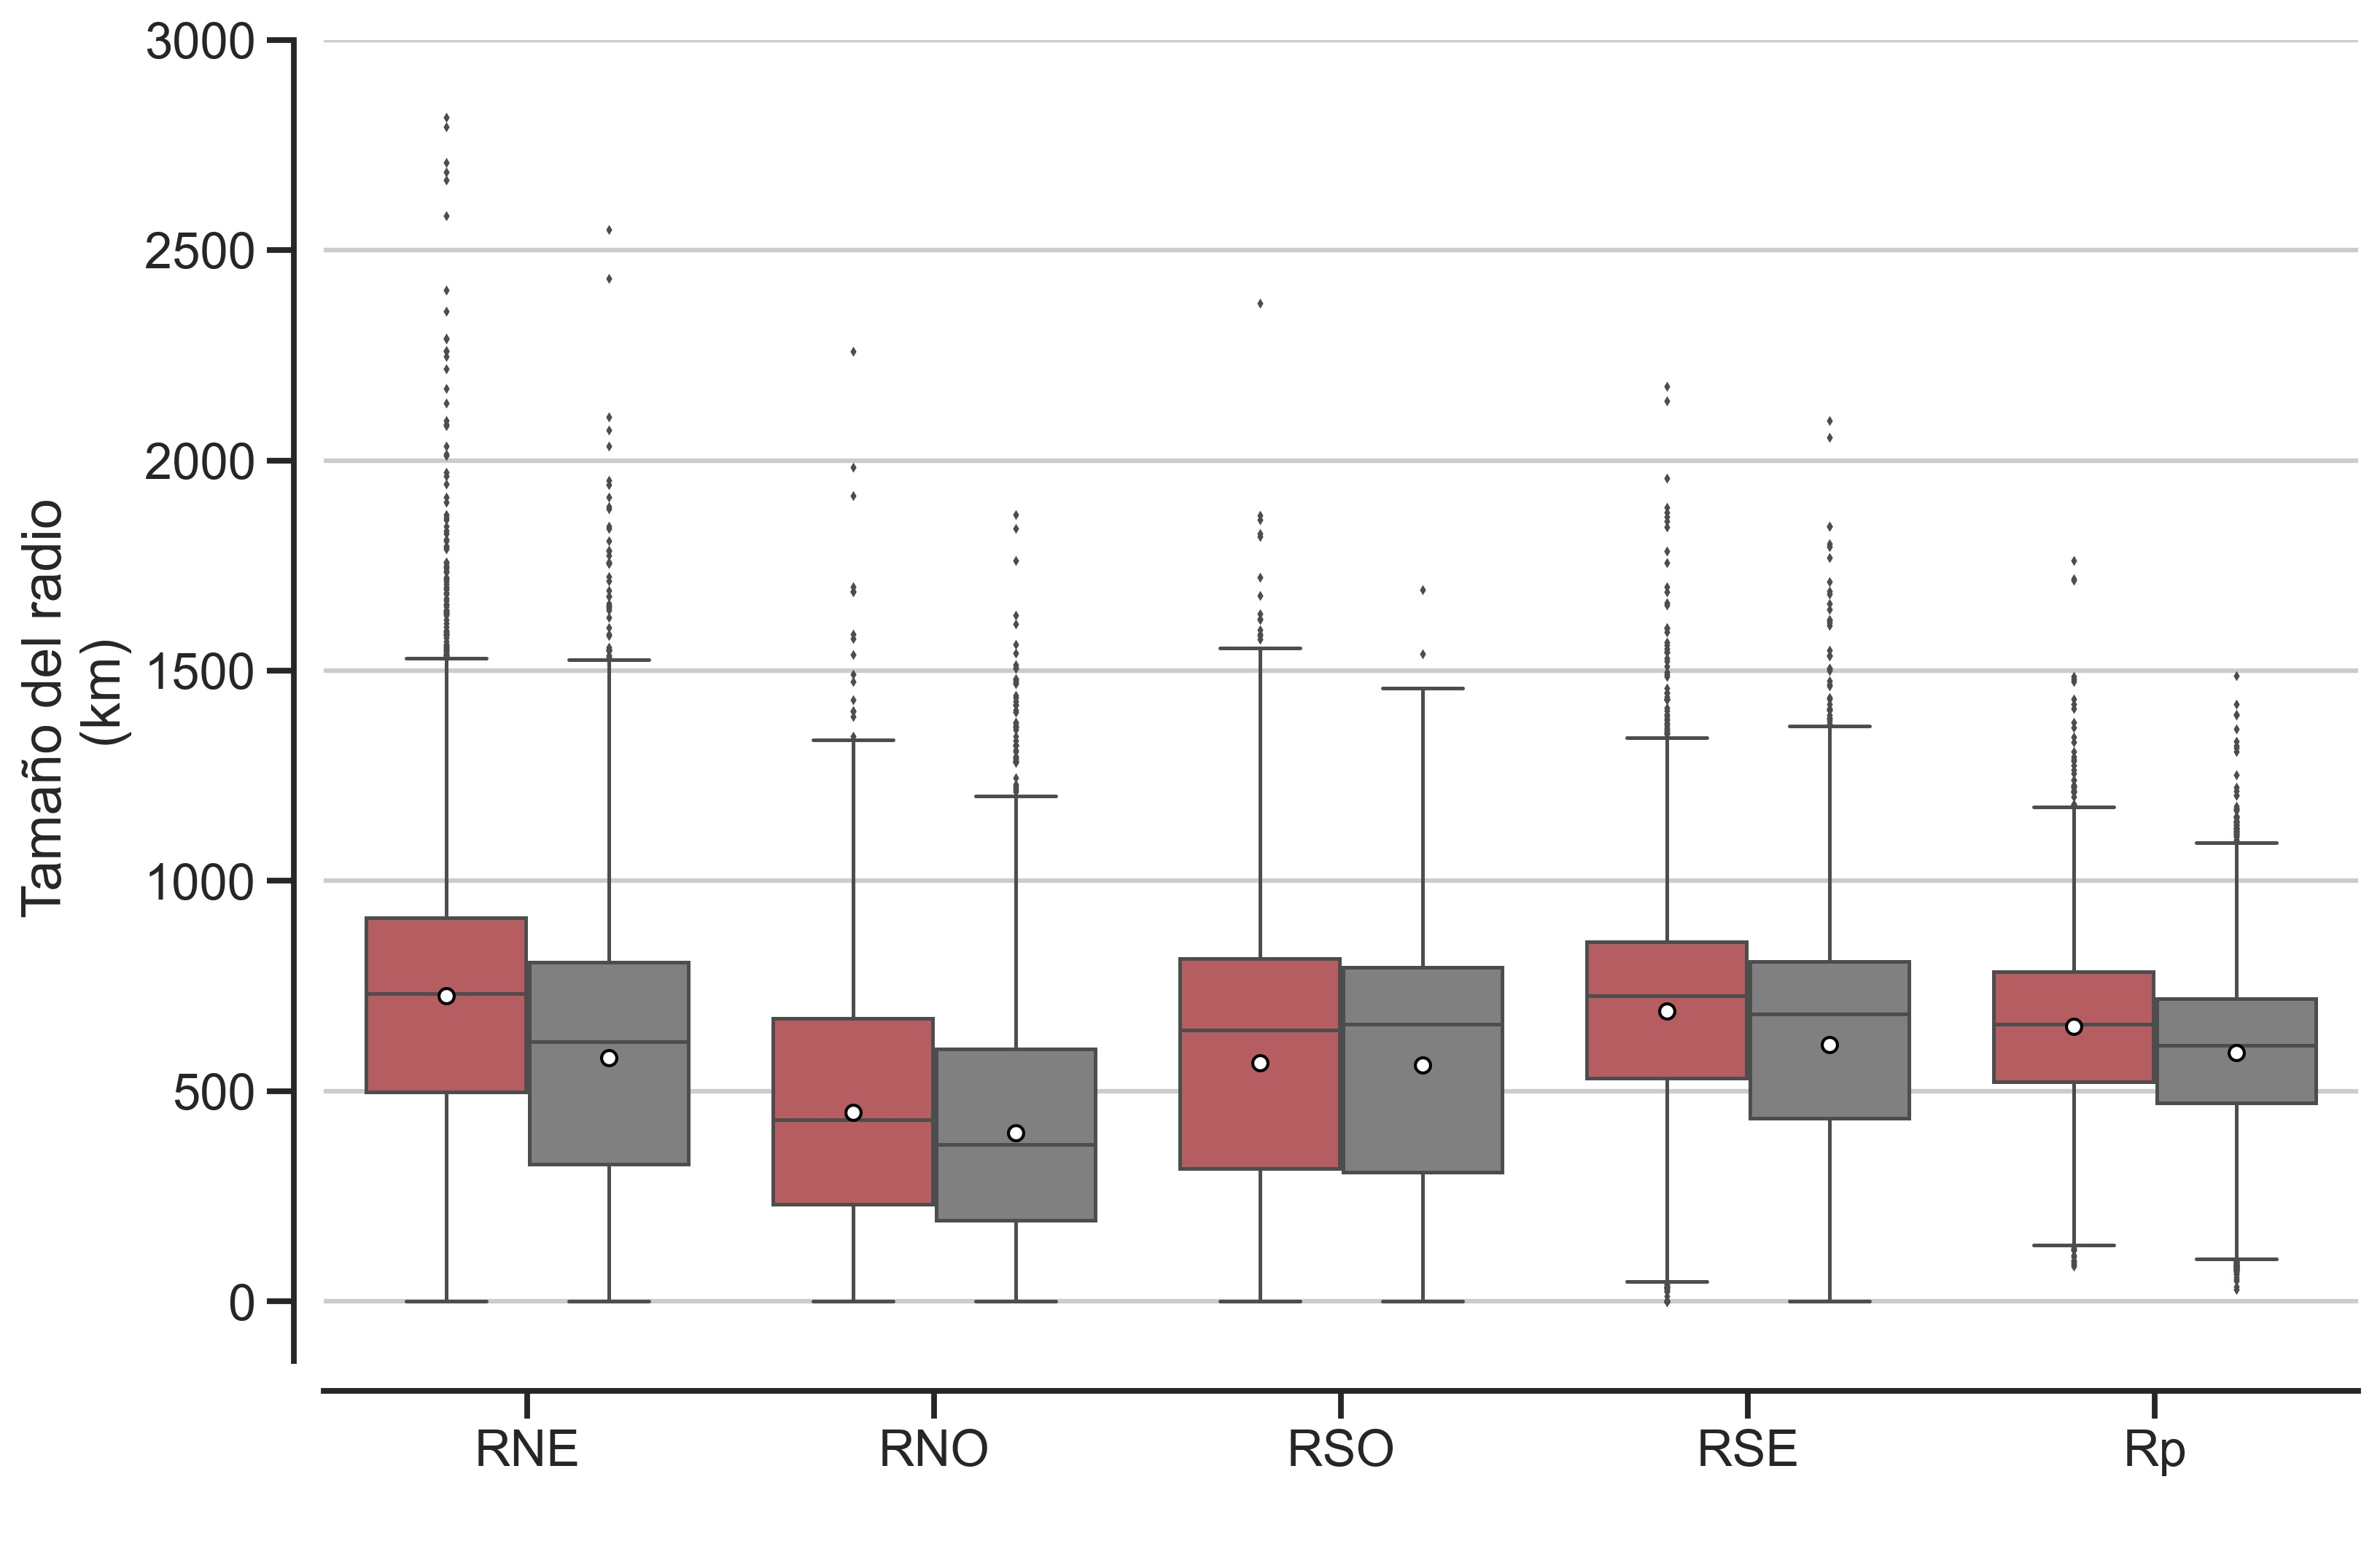
\includegraphics[scale = 0.35]{Images/Figures/Fig_3_1.jpeg}
        \caption{Cajas y bigotes de las distribuciones de los radios por cuadrante y el $R_p$ (km) de los radios en la región de estudio de la cuenca {\red NA} y {\gray EP}.}
        \label{fig:fig_9}
    \end{figure}
\end{frame}

\subsection{Sobre la relación del tamaño y la precipitación}
\begin{frame}

\end{frame}

\subsection{Sobre las variables medioambientales y la precipitación}
\begin{frame}
\begin{itemize}
    \item Algunos CT muestran una fuerte divergencia en la atmósfera superior. Puede estar relacionado con grandes cantidades de humedad en la atmósfera de nivel medio, lo que produce tasas de precipitación intensas de CT en la superficie.

    \item Los CTs en ambientes secos producen menos precipitación y tienen menores extensiones radiales de viento en comparación con los CTs en ambientes húmedos.

    \item La cizalladura del viento es más importante para los CT sobre la cuenca de {\red NA}. Esto último está posiblemente relacionado con el hecho de que las trayectorias de los CT cerca de la masa continental son modificadas por la cizalladura ambiental.

    \item Ni la intensidad del CT ni la presión central a nivel del mar son importantes para la estimación de la precipitación del CT, situado dentro del tamaño exterior del CT.
\end{itemize}
\end{frame}

\subsection{Sobre la forma del CT}
\begin{frame}
\begin{figure}
    \centering
    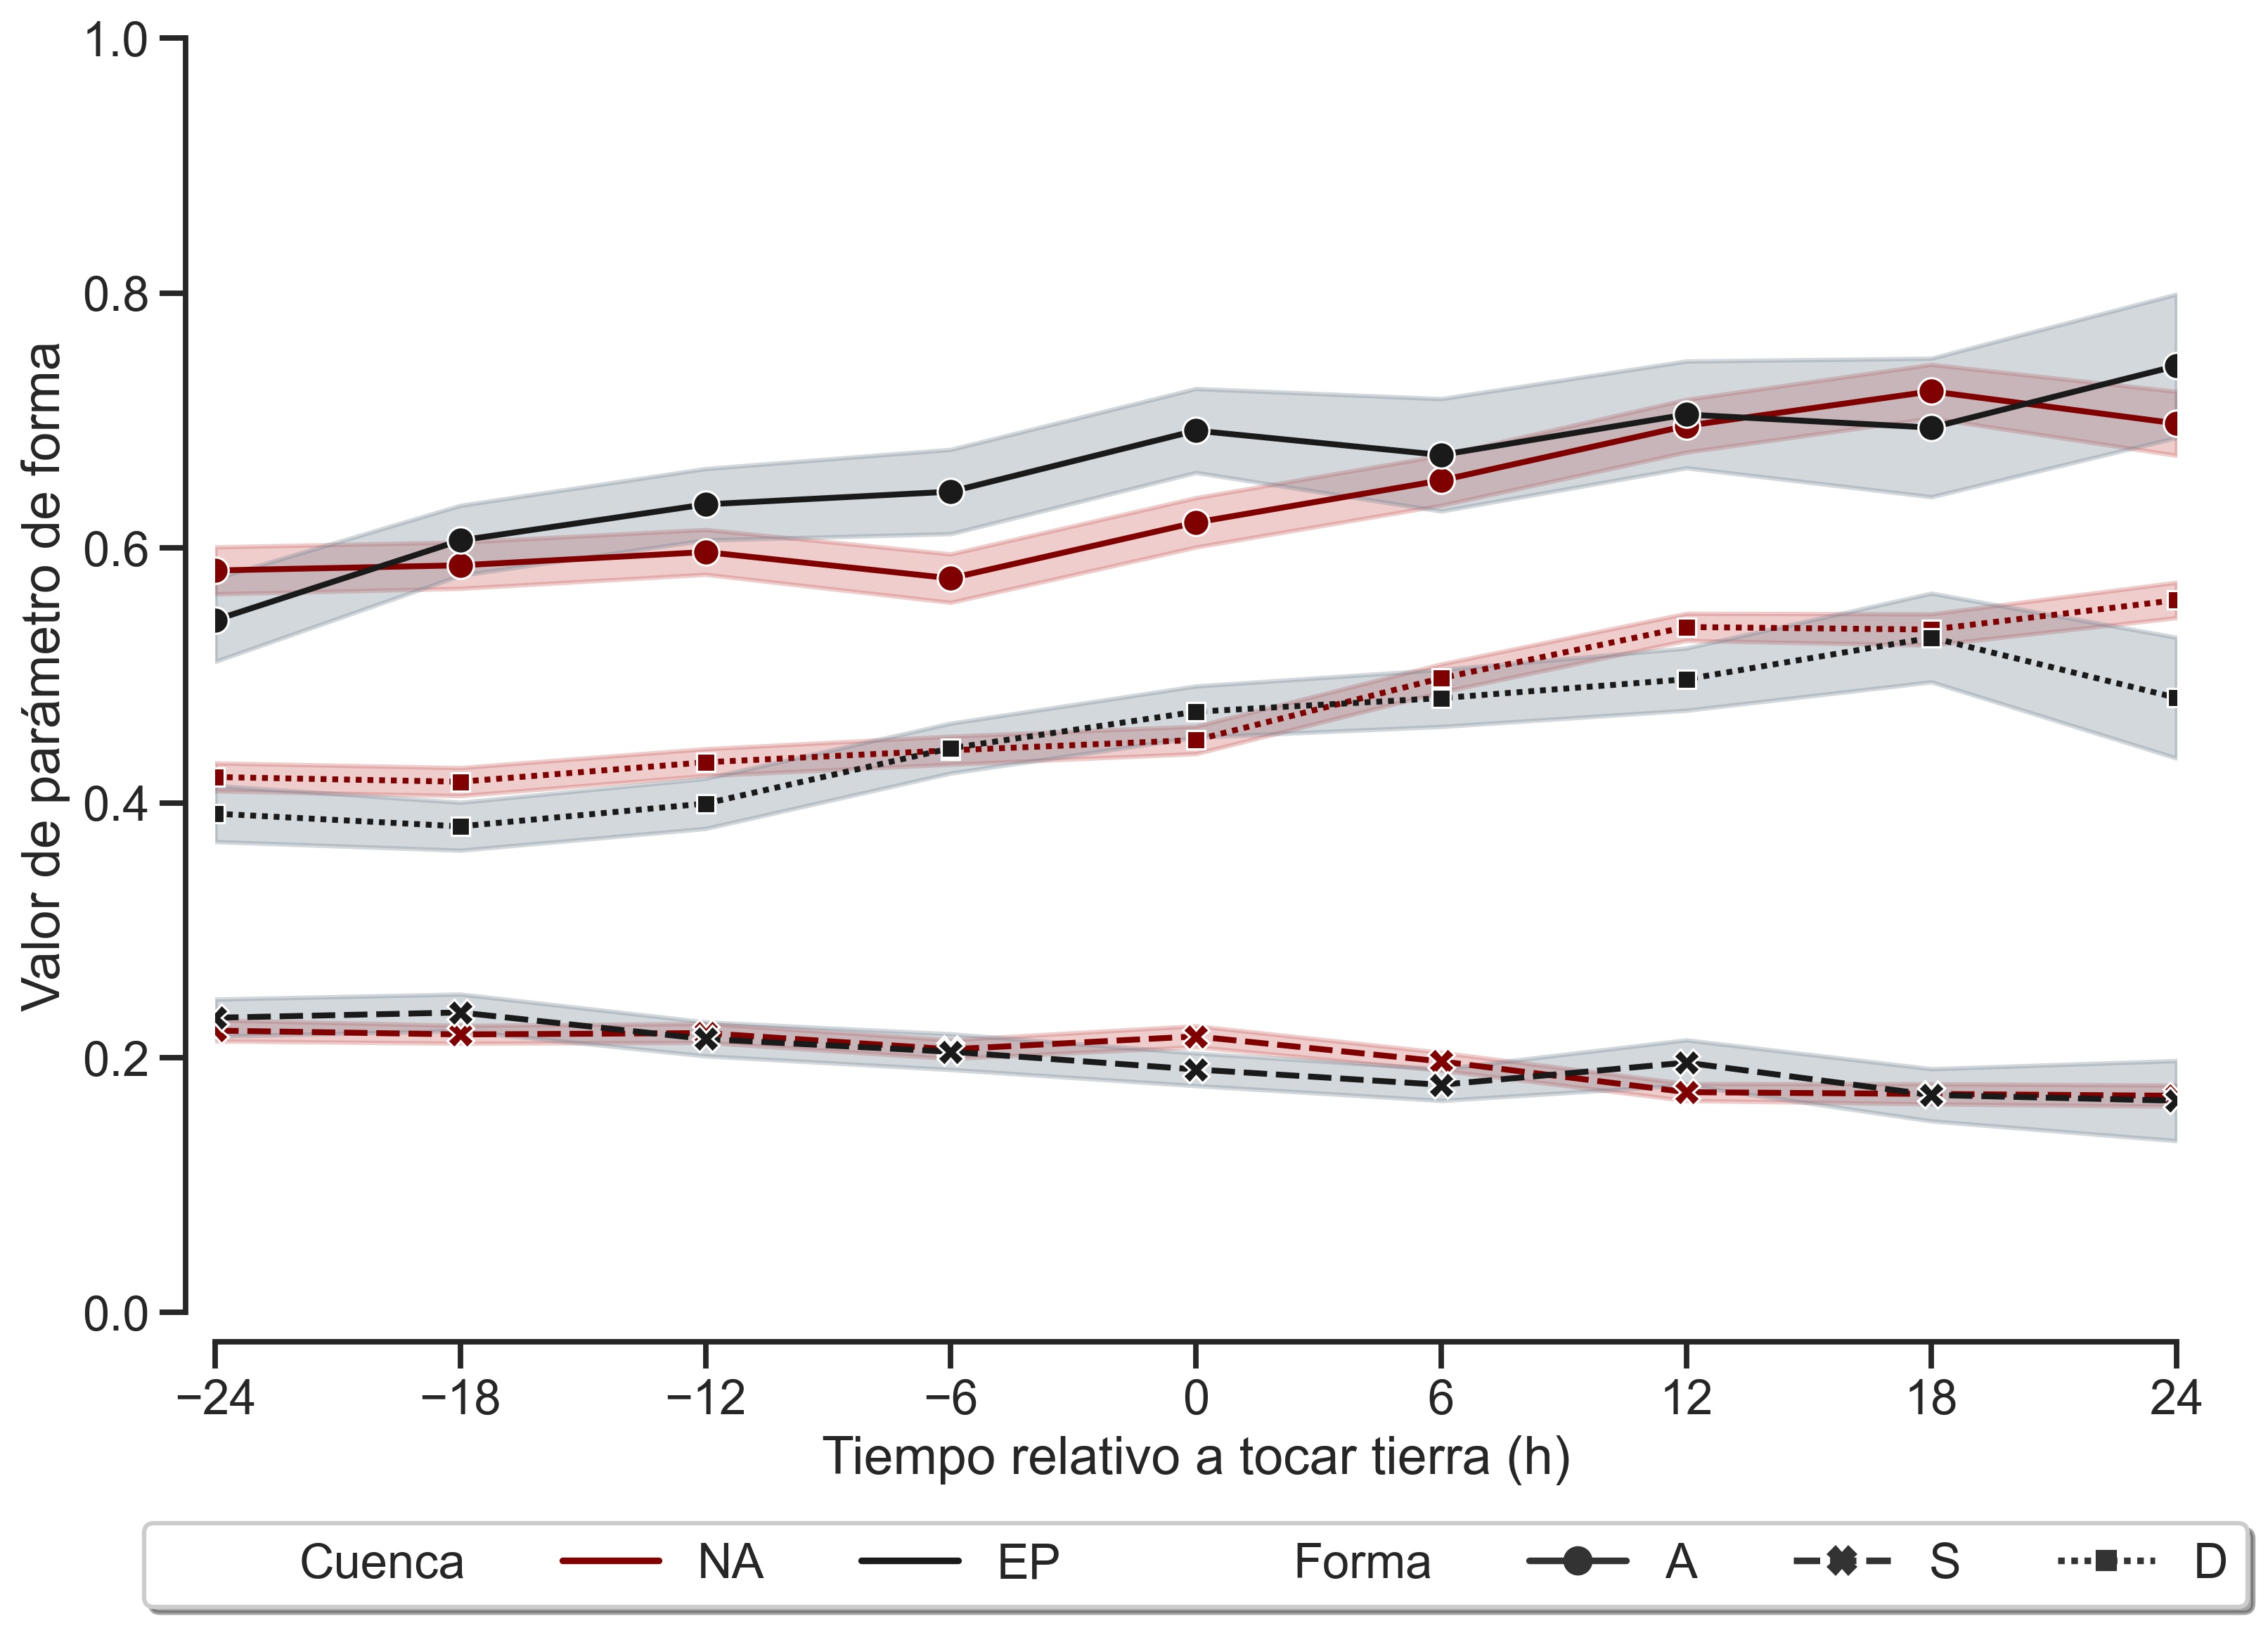
\includegraphics[scale = 0.3]{Images/Figures/Fig_3_32.jpeg}
    \caption{Comportamiento promedio de las métricas de forma de los CTs de la cuenca {\red NA} y {\gray EP}, 24h antes (-24) y 24h después (24) de hacer \textit{landfalling}.}
    \label{fig:fig_10}
\end{figure}
\end{frame}